% -*- mode: latex; -*- mustache tags:  
\documentclass[10pt,twoside,english]{_support/latex/sbabook/sbabook}
\let\wholebook=\relax

\usepackage{import}
\subimport{_support/latex/}{common.tex}

%=================================================================
% Debug packages for page layout and overfull lines
% Remove the showtrims document option before printing
\ifshowtrims
  \usepackage{showframe}
  \usepackage[color=magenta,width=5mm]{_support/latex/overcolored}
\fi


% =================================================================
\title{Learning Object-Oriented Programming, Design and TDD with Pharo}
\author{Stéphane Ducasse}
\series{The Pharo TextBook Collection}

\hypersetup{
  pdftitle = {Learning Object-Oriented Programming, Design and TDD with Pharo},
  pdfauthor = {Stéphane Ducasse},
  pdfkeywords = {Introduction, programming, design, testing, Pharo, Smalltalk}
}


% =================================================================
\begin{document}

% Title page and colophon on verso
\maketitle
\pagestyle{titlingpage}
\thispagestyle{titlingpage} % \pagestyle does not work on the first one…

\cleartoverso
{\small

  Copyright 2017 by Stéphane Ducasse.

  The contents of this book are protected under the Creative Commons
  Attribution-ShareAlike 3.0 Unported license.

  You are \textbf{free}:
  \begin{itemize}
  \item to \textbf{Share}: to copy, distribute and transmit the work,
  \item to \textbf{Remix}: to adapt the work,
  \end{itemize}

  Under the following conditions:
  \begin{description}
  \item[Attribution.] You must attribute the work in the manner specified by the
    author or licensor (but not in any way that suggests that they endorse you
    or your use of the work).
  \item[Share Alike.] If you alter, transform, or build upon this work, you may
    distribute the resulting work only under the same, similar or a compatible
    license.
  \end{description}

  For any reuse or distribution, you must make clear to others the
  license terms of this work. The best way to do this is with a link to
  this web page: \\
  \url{http://creativecommons.org/licenses/by-sa/3.0/}

  Any of the above conditions can be waived if you get permission from
  the copyright holder. Nothing in this license impairs or restricts the
  author's moral rights.

  \begin{center}
    
\includegraphics[width=0.2\textwidth]{_support/latex/sbabook/CreativeCommons-BY-SA.pdf}
  \end{center}

  Your fair dealing and other rights are in no way affected by the
  above. This is a human-readable summary of the Legal Code (the full
  license): \\
  \url{http://creativecommons.org/licenses/by-sa/3.0/legalcode}

  \vfill

  % Publication info would go here (publisher, ISBN, cover design…)
  Layout and typography based on the \textcode{sbabook} \LaTeX{} class by Damien
  Pollet.
}


\frontmatter
\pagestyle{plain}

\tableofcontents*
\clearpage\listoffigures

\mainmatter

\chapter{A simple network simulator }\label{ch:lan}
In this chapter, we develop a simulator for a computer network, step by step from scratch.
The program starts with a simplistic model of a computer network, made of objects that represent different parts of a local network such as packets, nodes, workstations, routers and hubs.

At first, we will just simulate the different steps of packet delivery and have fun with the system.
In a second step we will extend the basic functionalities by adding extensions such as a hub and different packet routing strategies.
Doing so, we will revisit many object-oriented concepts such as polymorphism, encapsulation, hooks and templates.
Finally this system could be refined to become an experiment platform to explore and understand distributed algorithms.


\begin{figure}

\begin{center}
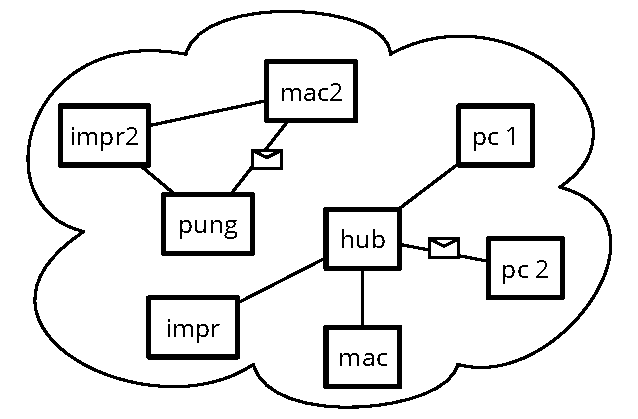
\includegraphics[width=0.8\textwidth]{/Users/ducasse/Workspace/FirstCircle/MyBooks/Bk-Writing/PharoBooks/LearningOOPWithPharoTrans/_result/pdf/Chapters/SimpleLAN/figures/lan-overview.pdf}\caption{Two little networks composed of nodes and sending packets over links.\label{/Users/ducasse/Workspace/FirstCircle/MyBooks/Bk-Writing/PharoBooks/LearningOOPWithPharoTrans/_result/pdf/Chapters/SimpleLAN/figures/lan-overview.pdf}}\end{center}
\end{figure}

\subsection{Basic definitions and a starting point}
We need to establish the basic model; what does the description above tell us?
A network is a number of interconnected nodes, which exchange data packets.
We will therefore probably need to model the nodes, the connection links, and the packets:

\begin{itemize}
\item Nodes have addresses, can send and receive packets;
\item Links connect two nodes together, and transmit packets between them;
\item A packet transports a payload and has the address of the node to which it should be delivered; if we want nodes to be able to answer (after reception), packets should also have the address of the node which originally sent it.
\end{itemize}
\section{Packets are simple value objects}
Packets seem to be the simplest objects in our model: we need to create them, and ask them about the data they contain, and that's about it.
Once created, a packet object is merely a passive data structure: it will not change its data, knows nothing of the surrounding network, and has no behavior that we can really talk about.

Let's start by defining a test class and a first test sketching what creating and looking at packets would look like:

\begin{displaycode}{smalltalk}
TestCase subclass: #KANetworkEntitiesTest
    instanceVariableNames: ''
    classVariableNames: ''
    category: 'NetworkSimulator-Tests'
\end{displaycode}

\begin{displaycode}{smalltalk}
KANetworkEntitiesTest >> testPacketCreation
    | src dest payload packet |
    src := Object new.
    dest := Object new.
    payload := Object new.

    packet := KANetworkPacket from: src to: dest payload: payload.

    self assert: packet sourceAddress equals: src.
    self assert: packet destinationAddress equals: dest.
    self assert: packet payload equals: payload
\end{displaycode}

By writing this unit test, we described how we think packets should be created, using a \textcode{from:to:payload:} constructor message, and how it should be accessed, using three messages \textcode{sourceAddress}, \textcode{destinationAddress}, and \textcode{payload}.
Since we have not yet decided what addresses and payloads should look like, we just pass arbitrary objects as parameters; all that matters is that when we ask the packet, it returns the correct object back.

Of course, if we now compile and run this test method, it will fail, because the class \textcode{KANetworkPacket} has not been created yet, nor any of the four above messages.
You can either execute and let the system prompt you when needed or we can define the class:

\begin{displaycode}{smalltalk}
Object subclass: #KANetworkPacket
    instanceVariableNames: 'sourceAddress destinationAddress payload'
    classVariableNames: ''
    category: 'NetworkSimulator-Core'
\end{displaycode}

The class-side constructor method creates an instance, which it returns after sending it an initialization message; nothing original as far as constructors go:

\begin{displaycode}{smalltalk}
KANetworkPacket class >> from: sourceAddress to: destinationAddress payload: anObject
    ... Your code ...
\end{displaycode}

That constructor will need to pass the initialization parameters to the new instance.
It's preferable to define a single initialization method that takes all needed parameters at once, since it is only supposed to be called when creating packets and should not be confused with a setter:

\begin{displaycode}{smalltalk}
KANetworkPacket >> initializeSource: source destination: destination payload: anObject
    ... Your code ...
\end{displaycode}

Once a packet is created, all we need to do with it is to obtain its payload, or the addresses of its source or destination nodes.
Define the following getters:

\begin{displaycode}{smalltalk}
KANetworkPacket >> sourceAddress
	... Your code ...
KANetworkPacket >> destinationAddress
	... Your code ...
KANetworkPacket >> payload
	... Your code ...
\end{displaycode}

Now our test should be running and passing.
That's enough for our admittedly simplistic model of packets; we completely ignore the layers of the OSI model, but it could be an interesting exercise to model them more precisely.
\section{Nodes are known by their address}
The first obvious thing we can say about a network node is that if we want to be able to send packets to it, then it should have an address; let's translate that into a test:

\begin{displaycode}{smalltalk}
KANetworkEntitiesTest >> testNodeCreation
    | address node |
    address := Object new.
    node := KANetworkNode withAddress: address.
    self assert: node address equals: address
\end{displaycode}

Like before, to run this test to completion, we will have to define the \textcode{KANetworkNode} class:

\begin{displaycode}{smalltalk}
Object subclass: #KANetworkNode
    instanceVariableNames: 'address'
    classVariableNames: ''
    category: 'NetworkSimulator-Core'
\end{displaycode}

Then a class-side constructor method taking the address of the new node as parameter:

\begin{displaycode}{smalltalk}
KANetworkNode class >> withAddress: aNetworkAddress
    ^ self new
        initializeAddress: aNetworkAddress;
        yourself
\end{displaycode}

The constructor relies on an instance-side initialization method, and the test asserts that the \textcode{address} accessor works; define them:

\begin{displaycode}{smalltalk}
KANetworkNode >> initializeAddress: aNetworkAddress
	... Your code ...
KANetworkNode >> address
	... Your code ...
\end{displaycode}

Again, our simplistic tests should now pass.
\section{Links are one-way connections between nodes}
After nodes and packets, what about looking at links?
In the real world, network cables are bidirectional, but that's because they have wires going both ways.
Here, we're going to keep it simple and define links as simple one-way connections; to make a two-way connection, we will just use two links, one in each direction.

However, creating links that know their source and destination nodes is not sufficient: \textit{nodes} also need to know about their outgoing links, otherwise they cannot send packets. Let us write a test to cover this.

\begin{displaycode}{smalltalk}
KANetworkEntitiesTest >> testNodeLinking
    | node1 node2 link |
    node1 := KANetworkNode withAddress: #address1.
    node2 := KANetworkNode withAddress: #address2.
    link := KANetworkLink from: node1 to: node2.

    link attach.

    self assert: (node1 hasLinkTo: node2)
\end{displaycode}

This test creates two nodes and a link; after telling the link to \textit{attach} itself, we check that it did so: the source node should confirm that it has an outgoing link to the destination node.
Note that the constructor could have registered the link with \textcode{node1}, but we opted for a separate message \textcode{attach} instead, because it's bad form to have a constructor change other objets; this way we can build links between arbitrary nodes and still have control of when the connection really becomes part of the network model.
For symmetry, we could have specified that \textcode{node2} has an incoming link from \textcode{node1}, but that ends up not being necessary, so we leave that out for now.

Again, we need to define the class of links:

\begin{displaycode}{smalltalk}
Object subclass: #KANetworkLink
    instanceVariableNames: 'source destination'
    classVariableNames: ''
    category: 'NetworkSimulator-Core'
\end{displaycode}

A constructor that passes the two required parameters to an instance-side initialization message:

\begin{displaycode}{smalltalk}
KANetworkLink class >> from: sourceNode to: destinationNode
    ^ self new
        initializeFrom: sourceNode to: destinationNode
\end{displaycode}

As well as the initialization method and accessors:

\begin{displaycode}{smalltalk}
KANetworkLink >> initializeFrom: sourceNode to: destinationNode
	... Your code ...
KANetworkLink >> source
	... Your code ...
KANetworkLink >> destination
	... Your code ...
\end{displaycode}

The \textcode{attach} method of a link should not (and cannot) directly modify the source node, so it must delegate to it instead.

\begin{displaycode}{smalltalk}
KANetworkLink >> attach
    source attach: self
\end{displaycode}

This is an example of separation of concerns: the link knows which node has to do what, but only the node itself knows precisely how to do that.
Here, if a node knows about all its outgoing links, it means it has a collection of those, and attaching a link adds it to that collection:

\begin{displaycode}{smalltalk}
KANetworkNode >> attach: anOutgoingLink
    outgoingLinks add: anOutgoingLink
\end{displaycode}

For this method to compile correctly, we will need to extend \textcode{KANetworkNode} with the new instance variable \textcode{outgoingLinks}, and with the corresponding initialization code:

\begin{displaycode}{smalltalk}
KANetworkNode >> initialize
    outgoingLinks := Set new.
\end{displaycode}

And finally the unit test relied on a predicate method to define in \textcode{KANetworkNode}:

\begin{displaycode}{smalltalk}
KANetworkNode >> hasLinkTo: anotherNode
    ... Your code ...
\end{displaycode}

The method \textcode{hasLinkTo:} should verify that there is at least one outgoing links whose destination is the node passed as argument.  We suggest to have a look at the iterator \textcode{anySatisfy:} to express this logic.

Again, all the tests should now pass.


\begin{figure}

\begin{center}
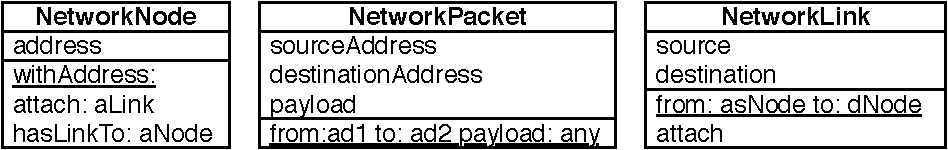
\includegraphics[width=0.8\textwidth]{/Users/ducasse/Workspace/FirstCircle/MyBooks/Bk-Writing/PharoBooks/LearningOOPWithPharoTrans/_result/pdf/Chapters/SimpleLAN/figures/API1.pdf}\caption{Current API of our three main classes.\label{/Users/ducasse/Workspace/FirstCircle/MyBooks/Bk-Writing/PharoBooks/LearningOOPWithPharoTrans/_result/pdf/Chapters/SimpleLAN/figures/API1.pdf}}\end{center}
\end{figure}

\section{Making our objects more understandable}
When programming we often make mistakes and it is important to help developer to address them. Let us put a breakpoint and 
try to understand the objects. 

\begin{displaycode}{smalltalk}
KANetworkEntitiesTest >> testNodeLinking
	| node1 node2 link |
	node1 := KANetworkNode withAddress: #address1.
	node2 := KANetworkNode withAddress: #address2.
	link := KANetworkLink from: node1 to: node2.
	link attach.
	self halt.
	self assert: (node1 hasLinkTo: node2)
\end{displaycode}

Running the test will open a debugger as the one shown in Figure \ref{debugger}. We get object but their textual representation is too generic to really help us. 


\begin{figure}

\begin{center}
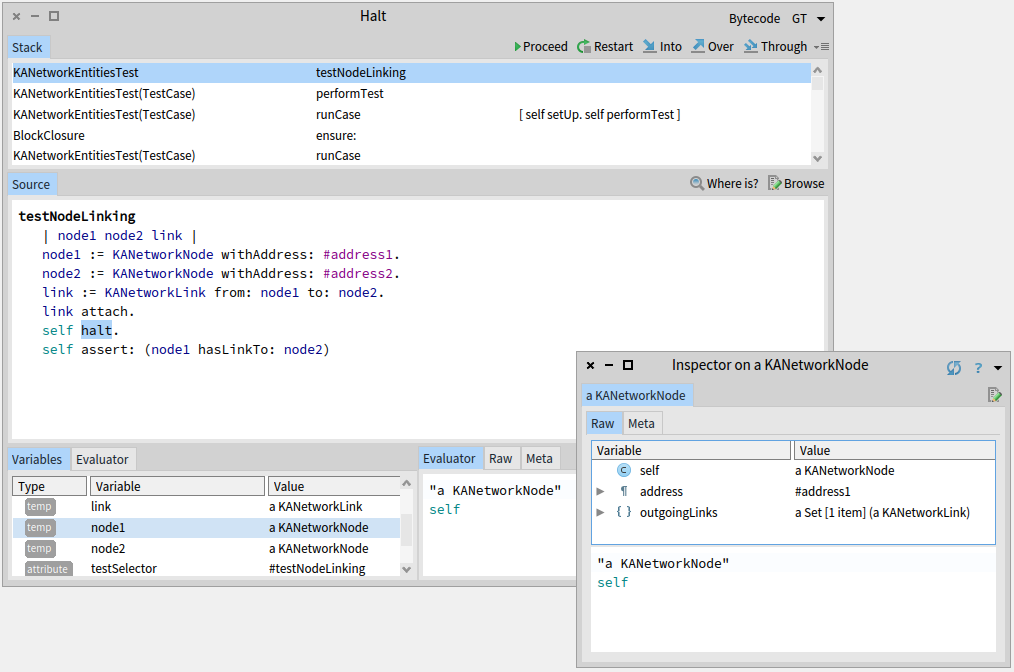
\includegraphics[width=1.0\textwidth]{/Users/ducasse/Workspace/FirstCircle/MyBooks/Bk-Writing/PharoBooks/LearningOOPWithPharoTrans/_result/pdf/Chapters/SimpleLAN/figures/debugger.png}\caption{Navigating specific objects having a generic presentation.\label{debugger}}\end{center}
\end{figure}


The method \textcode{printOn:} is responsible to the printing of the object representation. We will then redefine this method for the different objects we have.

\begin{displaycode}{smalltalk}
KANetworkNode >> printOn: aStream
	aStream nextPutAll: 'Node ('.
	aStream nextPutAll: address , ')'
\end{displaycode}

\begin{displaycode}{smalltalk}
KANetworkLink >> printOn: aStream
	aStream nextPutAll: 'Link'.
	source
		ifNotNil: [ aStream
				nextPutAll: ' ';
				nextPutAll: source address ].
	destination
		ifNotNil: [ aStream
				nextPutAll: ' -> ';
				nextPutAll: destination address ]
\end{displaycode}

Now if we rerun the test we obtain a better user experience as shown in Figure \ref{debuggerXP}: we can see the address of a node and the source and destination of a link.


\begin{figure}

\begin{center}
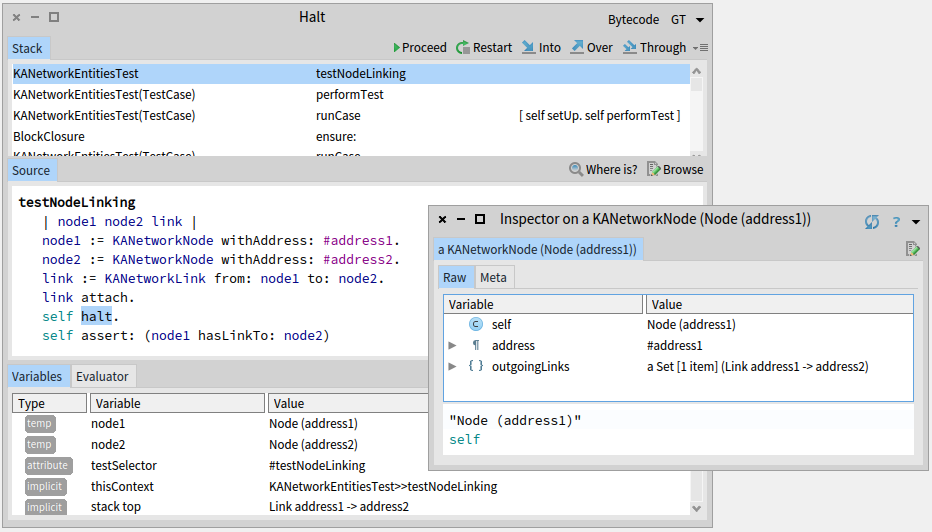
\includegraphics[width=1.0\textwidth]{/Users/ducasse/Workspace/FirstCircle/MyBooks/Bk-Writing/PharoBooks/LearningOOPWithPharoTrans/_result/pdf/Chapters/SimpleLAN/figures/betterDebugerXP.png}\caption{Navigating objects offering a customized presentation.\label{debuggerXP}}\end{center}
\end{figure}

\section{Simulating the steps of packet delivery}
The next big feature is that nodes should be able to send and receive packets, and links to transmit them.

\begin{displaycode}{smalltalk}
KANetworkEntitiesTest >> testSendAndTransmit
    | srcNode destNode link packet |
    srcNode := KANetworkNode withAddress: #src.
    destNode := KANetworkNode withAddress: #dest.
    link := (KANetworkLink from: srcNode to: destNode) attach; yourself.
    packet := KANetworkPacket from: #address to: #dest payload: #payload.

    srcNode send: packet via: link.
    self assert: (link isTransmitting: packet).
    self deny: (destNode hasReceived: packet).

    link transmit: packet.
    self deny: (link isTransmitting: packet).
    self assert: (destNode hasReceived: packet)
\end{displaycode}

We create and setup two nodes, a link between them, and a packet.
Now, to control which packets get delivered in which order, we specify that it happens in separate, controlled steps.
This will allow us to model packet delivery precisely, to simulate latency, out-of-order reception, etc.:

\begin{itemize}
\item First, we tell the node to send the packet using the message \textcode{send:via:}. At that point, the packet should be passed to the link for transmission, but not completely delivered yet.
\item Then, we tell the link to actually transmit the packet along using the message \textcode{transmit:}, and thus the packet should be received by the destination node.
\end{itemize}
\section{Sending a packet}
To send a packet, the node emits it on the link:

\begin{displaycode}{smalltalk}
KANetworkNode >> send: aPacket via: aLink
    aLink emit: aPacket
\end{displaycode}

For the simulation to be realistic, we do not want the packet to be delivered right away; instead, emitting a packet really just stores it in the link, until the user elects this packet to proceed using the \textcode{transmit:} message.
Storing packets requires adding an instance variable to \textcode{KANetworkLink}, as well as specifying how this instance variable should be initialized.

\begin{displaycode}{smalltalk}
Object subclass: #KANetworkLink
    instanceVariableNames: 'source destination packetsToTransmit'
    classVariableNames: ''
    category: 'NetworkSimulator-Core'
\end{displaycode}

\begin{displaycode}{smalltalk}
KANetworkLink >> initialize
    packetsToTransmit := OrderedCollection new
\end{displaycode}

\begin{displaycode}{smalltalk}
KANetworkLink >> emit: aPacket
    "Packets are not transmitted right away, but stored.
    Transmission is explicitly triggered later, by sending #transmit:."
	
    packetsToTransmit add: aPacket
\end{displaycode}

We also add a testing method to check whether a given packet is currently being transmitted by a link:

\begin{displaycode}{smalltalk}
KANetworkLink >> isTransmitting: aPacket
    ... Your code ...
\end{displaycode}
\section{Transmitting across a link}
Transmitting a packet means telling the link's destination node to receive it. Nodes only consume packets addressed to them; fortunately this is what will happen in our test, so we can worry about the alternative case later (\textcode{notYetImplemented} is a special message that we can use in place of code that we will have to write eventually, but prefer to ignore for now).

\begin{displaycode}{smalltalk}
KANetworkNode >> receive: aPacket from: aLink
    aPacket destinationAddress = address
        ifTrue: [
            self consume: aPacket.
            arrivedPackets add: aPacket ]
        ifFalse: [ self notYetImplemented ]
\end{displaycode}

Consuming a packet represents what the node will do with it at the application level; for now let's just define an empty \textcode{consume:} method, as a placeholder:

\begin{displaycode}{smalltalk}
KANetworkNode >> consume: aPacket
    "Default handling is to do nothing."
\end{displaycode}

After consuming the packet, we remember it did arrive; this is mostly for testing and debugging, but someday we might want to simulate packet losses and re-emissions.
Don't forget to declare and initialize the \textcode{arrivedPackets} instance variable, along with its accessor:

\begin{displaycode}{smalltalk}
KANetworkNode >> hasReceived: aPacket
	... Your code ...
\end{displaycode}

Now we can implement the \textcode{transmit:} message. A link can not transmit packets that have not been sent via it, and once transmitted, the packet should not be on the link anymore. We should remove it from the link list of package to be transmitted
and tell the destination to receive it using the message \textcode{receive:from:}.

\begin{displaycode}{smalltalk}
KANetworkLink >> transmit: aPacket
    "Transmit aPacket to the destination node of the receiver link."
    ... Your code ...
\end{displaycode}

At that point all our tests should pass.
Note that the message \textcode{notYetImplemented} is not called, since our tests do not yet require routing.
Figure \ref{Api2} shows that the API of our classes is getting richer than before. 


\begin{figure}

\begin{center}
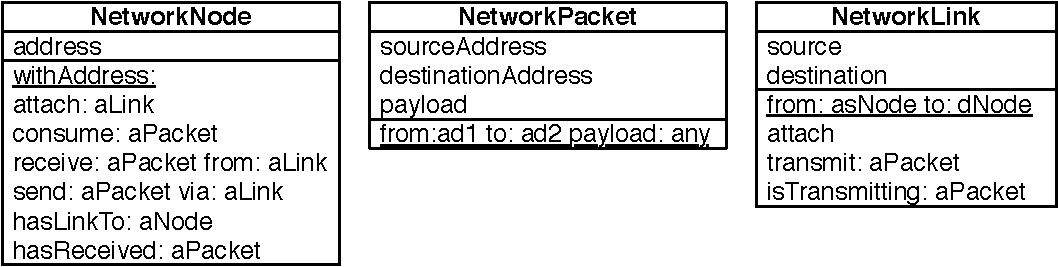
\includegraphics[width=0.9\textwidth]{/Users/ducasse/Workspace/FirstCircle/MyBooks/Bk-Writing/PharoBooks/LearningOOPWithPharoTrans/_result/pdf/Chapters/SimpleLAN/figures/API2.pdf}\caption{Richer API.\label{Api2}}\end{center}
\end{figure}

\section{The loopback link}
On a real network, when a node wants to send a packet to itself, it does not need any connection to do so.
In real-world networking stacks, loopback routing shortcuts the lower networking layers; however, this is finer detail than we are modeling here.

Still, we want to model the fact that the loopback link is a little special, so each node will store its own loopback link, separately from the outgoing links. We start to define a test. 

\begin{displaycode}{smalltalk}
KANetworkEntitiesTest >> testLoopback
    | node packet |
    node := KANetworkNode withAddress: #address.
    packet := KANetworkPacket from: #address to: #address payload: #payload.

    node send: packet.
    node loopback transmit: packet.

    self assert: (node hasReceived: packet).
    self deny: (node loopback isTransmitting: packet)
\end{displaycode}

The loopback link is implicitely created as part of the node itself.
We also introduce a new \textcode{send:} message, which takes the responsibility of selecting the link to emit the packet.
For triggering packet transmission, we have to use a specific accessor to find the loopback link of the node.

First, we have to add yet another instance variable in nodes:

\begin{displaycode}{smalltalk}
Object subclass: #KANetworkNode
    instanceVariableNames: 'address outgoingLinks loopback arrivedPackets'
    classVariableNames: ''
    category: 'NetworkSimulator-Core'
\end{displaycode}

As with all instance variables, we have to remember to make sure it is correctly initialized; we thus modify \textcode{initialize}:

\begin{displaycode}{smalltalk}
KANetworkNode >> initialize
    ... Your code ...
\end{displaycode}

The accessor has nothing special:

\begin{displaycode}{smalltalk}
KANetworkNode >> loopback
    ^ loopback
\end{displaycode}

And finally we can focus on the \textcode{send:} method and automatic link selection. The method \textcode{send:} should be more generic than the method \textcode{send:via:} and will be one exposed as a public entry point.

This method has to rely on some routing algorithm to identify which links will transmit the packet closer to its destination.
Since some routing algorithms select more than one link, we will implement routing as an \textit{iteration} method, which evaluates the given block for each selected link.

\begin{displaycode}{smalltalk}
KANetworkNode >> send: aPacket
    "Send aPacket, leaving the responsibility of routing to the node."
    self
        linksTowards: aPacket destinationAddress
        do: [ :link | self send: aPacket via: link ]
\end{displaycode}

One of the simplest routing algorithm is \textit{flooding}: just send the packet via every outgoing link.
Obviously, this is a waste of bandwidth, but it works without any knowledge of the network topology beyond the list of outgoing links.

However, there is one case where we know how to route the packet: if the destination address matches the one of the current node, we can select the loopback link.
The logic of \textcode{linksTowards:do:} is then: compare the packet's destination address with the one of the node, if it is the same, we execute the block using the loopback link, else we simply iterate on the outgoing links of the receiver.

\begin{displaycode}{smalltalk}
KANetworkNode >> linksTowards: anAddress do: aBlock
    "Simple flood algorithm: route via all outgoing links.
    However, just loopback if the receiver node is the routing destination."
    ... Your code ...
\end{displaycode}

Now we have the basic model working, and we can try more realistic examples.
\section{Modeling the network itself}
More realistic tests will require non-trivial networks.
We thus need an object that represents the network as a whole, to avoid keeping many nodes and links in individual variables.
We will introduce a new class \textcode{KANetwork}, whose responsibility is to help us build, assemble then find the nodes and links involved in a network.

Let's start by creating another test class, to keep things in order:

\begin{displaycode}{smalltalk}
TestCase subclass: #KANetworkTest
    instanceVariableNames: 'net hub alone'
    classVariableNames: ''
    category: 'NetworkSimulator-Tests'
\end{displaycode}

Since every test needs to rebuild the whole example network from scratch, we specify so in the \textcode{setUp} method:

\begin{displaycode}{smalltalk}
KANetworkTest >> setUp
    self buildNetwork
\end{displaycode}

Before anything else, let's write a test that will pass once we've made progress; we want to access network nodes given only their addresses. Here we check that we get a hub node based on its address: 

\begin{displaycode}{smalltalk}
KANetworkTest >> testNetworkFindsNodesByAddress
    self
        assert: (net nodeAt: hub address ifNone: [ self fail ])
        equals: hub
\end{displaycode}

We will have to implement this \textcode{nodeAt:ifNone:} on our \textcode{KANetwork} class; but first we need to decide how its instances are built.
Let's build network \textcode{net}, with the main part connected in a star shape around a \textcode{hub} node; a pair of nodes \textcode{ping} and \textcode{pong} are part of the network but not connected to \textcode{hub}, and the \textcode{alone} node is just by itself, not even added to the network as shown in Figure \ref{hub}.


\begin{figure}

\begin{center}
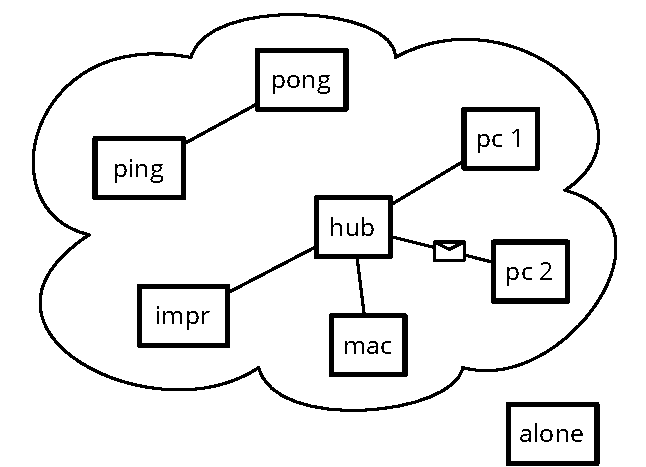
\includegraphics[width=0.5\textwidth]{/Users/ducasse/Workspace/FirstCircle/MyBooks/Bk-Writing/PharoBooks/LearningOOPWithPharoTrans/_result/pdf/Chapters/SimpleLAN/figures/lan-star.pdf}\caption{A hub.\label{hub}}\end{center}
\end{figure}


Expanding a network implies adding new connections and possibly new nodes to it.
If the \textcode{net} object understands a \textcode{connect: aNode to: anotherNode} message, you should be able to build nodes and connect them into a network that matches the figure.

\begin{displaycode}{smalltalk}
KANetworkTest >> buildNetwork
	alone := KANetworkNode withAddress: #alone.
	net := KANetwork new.
	hub := KANetworkNode withAddress: #hub.
	#(mac pc1 pc2 prn)
		do: [ :addr | 
			| node |
			node := KANetworkNode withAddress: addr.
			net connect: node to: hub ].
	net connect: (KANetworkNode withAddress: #ping) to: (KANetworkNode withAddress: #pong)
\end{displaycode}

The name of the \textcode{connect:to:} message suggests that establishing the bidirectional links is the responsibility of the \textcode{net} object. It also has to remember enough info so we can inspect the network topology; we can simply store nodes and links in a couple of sets, even though that representation is a little redundant.
Let's define the class with two instance variables:

\begin{displaycode}{smalltalk}
Object subclass: #KANetwork
    instanceVariableNames: 'nodes links'
    classVariableNames: ''
    category: 'NetworkSimulator-Core'
\end{displaycode}

Whenever we define an instance variable, initialization comes next:

\begin{displaycode}{smalltalk}
KANetwork >> initialize
    ... Your code ...
\end{displaycode}

Now we can give the network the possibility to create links.  This method we will use to add links to the network link collection.

\begin{displaycode}{plain}
KANetwork >> makeLinkFrom: aNode to: anotherNode
	^ KANetworkLink from: aNode to: anotherNode
\end{displaycode}

We add a low level method \textcode{add:} to add a node in a network. 

\begin{displaycode}{smalltalk}
KANetwork >> add: aNode
	nodes add: aNode
\end{displaycode}

To be able to test the network construction we add a little test message;

\begin{displaycode}{smalltalk}
KANetwork >> doesRecordNode: aNode
	^ nodes includes: aNode
\end{displaycode}

Now, we can add isolated nodes to the network, even if it does not seem very useful.
\subsection{Connecting nodes.}
Connecting nodes without ensuring that they are part of the network really does not make sense.
Therefore, when connecting nodes, we will first ensure the nodes are added (by simply adding them in the node Set of the network), then we create and attach links in \textit{both} directions; finally we store both links.

Here is a test covering this aspect.

\begin{displaycode}{plain}
KANetworkTest >> testConnect
	| netw hubb mac pc1 |
	netw := KANetwork new.
	hubb := KANetworkNode withAddress: #hub.
	mac := KANetworkNode withAddress: #mac.
	pc1 := KANetworkNode withAddress: #pc1.

	netw connect: hubb to: mac.
	self assert: (hubb hasLinkTo: mac).
	self assert: (mac hasLinkTo: hubb).
	self assert: (netw doesRecordNode: hubb).
	self assert: (netw doesRecordNode: mac).

	netw connect: hubb to: pc1.
	self assert: (hubb hasLinkTo: pc1).
	self assert: (mac hasLinkTo: hubb)
\end{displaycode}

Now implement the \textcode{connect:to:} method; for concision, note that the \textcode{attach} method we defined previously effectively returns the link.

\begin{displaycode}{smalltalk}
KANetwork >> connect: aNode to: anotherNode
    ... Your code ...
\end{displaycode}

The test \textcode{testConnect} should be green.
\section{Looking up nodes}
At this point, the test \textcode{testNetworkFindsNodesByAddress} should run through \textcode{setUp} but fail in the unit test itself, because we still need to implement node lookup. The base lookup should find the first node that has the requested address, or evaluate a fall-back block (a perfect case for the \textcode{detect:ifNone:} message):

\begin{displaycode}{smalltalk}
KANetwork >> nodeAt: anAddress ifNone: noneBlock
    ... Your code ...
\end{displaycode}

We can also make a convenience \textcode{nodeAt:} method for node lookup, that will raise the predefined \textcode{NotFound} exception if it does not find the node.
Let's first write a test which validates this behavior:

\begin{displaycode}{smalltalk}
KANetworkTest >> testNetworkOnlyFindsAddedNodes
    self
        should: [ net nodeAt: alone address ]
        raise: NotFound
\end{displaycode}

Then we can simply express \textcode{nodeAt:} by delegating to \textcode{nodeAt:ifNone:}.
Note that raise an exception, you simply send the message \textcode{signal} to the exception class. Here we use
the specific class method \textcode{signalFor:in:} defined on the \textcode{NotFound} class.

\begin{displaycode}{smalltalk}
KANetwork >> nodeAt: anAddress
    ^ self
        nodeAt: anAddress
        ifNone: [ NotFound signalFor: anAddress in: self ]
\end{displaycode}
\section{Looking up links}
Next, we want to be able to lookup links between two nodes.
Again we define a new test:

\begin{displaycode}{smalltalk}
KANetworkTest >> testNetworkFindsLinks
    | link |
    self
        shouldnt: [ link := net linkFrom: #pong to: #ping ]
        raise: NotFound.
    self
        assert: link source
        equals: (net nodeAt: #pong).
    self
        assert: link destination
        equals: (net nodeAt: #ping)
\end{displaycode}

And we define the method \textcode{linkFrom:to:} returning the link between source and destination nodes with matching addresses, and signalling \textcode{NotFound} if no such link is found:

\begin{displaycode}{smalltalk}
KANetwork >> linkFrom: sourceAddress to: destinationAddress
    ... Your code ...
\end{displaycode}
\subsection{Final check. }
As a final check, let's try some of the previous tests, first on the isolated \textcode{alone} node, showing that loopback works even without a network connection:

\begin{displaycode}{smalltalk}
KANetworkTest >> testSelfSend
    | packet |
    packet := KANetworkPacket
        from: alone address
        to: alone address
        payload: #something.
    self assert: (packet isAddressedTo: alone).
    self assert: (packet isOriginatingFrom: alone).

    alone send: packet.
    self deny: (alone hasReceived: packet).
    self assert: (alone loopback isTransmitting: packet).

    alone loopback transmit: packet.
    self deny: (alone loopback isTransmitting: packet).
    self assert: (alone hasReceived: packet)
\end{displaycode}

You can see that we used new convenience testing methods \textcode{isAddressedTo:} and \textcode{isOriginatingFrom:} which help inspect the state of a simulated network without explicitly comparing addresses.
However, those methods should not take part in network simulation code, since in the real world nodes can never know their peers other than through their addresses.

\begin{displaycode}{smalltalk}
KANetworkPacket >> isAddressedTo: aNode
    ^ destinationAddress = aNode address
\end{displaycode}

\begin{displaycode}{smalltalk}
KANetworkPacket >> isOriginatingFrom: aNode
    ^ sourceAddress = aNode address
\end{displaycode}

The second test attempts transmitting a packet in the network, between the directly connected nodes \textcode{ping} and \textcode{pong}:

\begin{displaycode}{smalltalk}
KANetworkTest >> testDirectSend
    | packet ping pong link |
    packet := KANetworkPacket from: #ping to: #pong payload: #ball.
    ping := net nodeAt: #ping.
    pong := net nodeAt: #pong.
    link := net linkFrom: #ping to: #pong.

    ping send: packet.
    self assert: (link isTransmitting: packet).
    self deny: (pong hasReceived: packet).

    link transmit: packet.
    self deny: (link isTransmitting: packet).
    self assert: (pong hasReceived: packet)
\end{displaycode}

Both tests should pass with no additional work, since they just reproduce what we already tested in \textcode{KANetworkEntitiesTest} and adding \textcode{KANetwork} did not impact the established behavior of nodes, links, and packets.
\section{Packet delivery with forwarding}
Until now, we only tested packet delivery between directly connected nodes; let's try sending a node so that the packet has to be forwarded through the hub.

\begin{displaycode}{smalltalk}
KANetworkTest >> testSendViaHub
    | hello mac pc1 firstLink secondLink |
    hello := KANetworkPacket from: #mac to: #pc1 payload: 'Hello!'.
    mac := net nodeAt: #mac.
    pc1 := net nodeAt: #pc1.
    firstLink := net linkFrom: #mac to: #hub.
    secondLink := net linkFrom: #hub to: #pc1.

    self assert: (hello isAddressedTo: pc1).
    self assert: (hello isOriginatingFrom: mac).

    mac send: hello.
    self deny: (pc1 hasReceived: hello).
    self assert: (firstLink isTransmitting: hello).

    firstLink transmit: hello.
    self deny: (pc1 hasReceived: hello).
    self assert: (secondLink isTransmitting: hello).

    secondLink transmit: hello.
    self assert: (pc1 hasReceived: hello).
\end{displaycode}

If you run this test, you will see that it fails because of the \textcode{notYetImplemented} message we left earlier in \textcode{receive:from:}; it's time to fix that!
When a node receives a packet but is not the recipient, it should forward the packet:

\begin{displaycode}{smalltalk}
KANetworkNode >> receive: aPacket from: aLink
    aPacket destinationAddress = address
        ifTrue: [
            self consume: aPacket.
            arrivedPackets add: aPacket ]
        ifFalse: [ self forward: aPacket from: aLink ]
\end{displaycode}

Now we need to implement packet forwarding, but there is a trap.
An easy solution would be to simply \textcode{send:} the packet again: the hub would send the packet to all its connected nodes, one of which happens to be \textcode{pc1}, the recipient, so all is good!

\textit{Wrong…}

The packet would be also sent to other nodes than the recipient; what would those nodes do when they receive a packet not addressed to them? Forward it. Where? To all their neighbours, which would forward it again... so when would the forwarding stop?

To fix this, we need hubs to behave differently from nodes.
In reality, hubs work at the lower layers of the OSI model, but our simplified model does not have that level of detail.
We can approximate this by saying that upon reception of a packet addressed to another node, a hub should forward the packet, but a normal node should just ignore it.

Let's first define an empty \textcode{forward:from:} method for nodes, then add a new class for hubs, which will be modeled as nodes with an actual implementation of forwarding:

\begin{displaycode}{smalltalk}
KANetworkNode >> forward: aPacket from: arrivalLink
    "Do nothing. Normal nodes do not route packets."
\end{displaycode}
\section{Introducing a new kind of node}
Now we define the class \textcode{KANetworkHub} that will be the recipient of hub specific behavior. 

\begin{displaycode}{smalltalk}
KANetworkNode subclass: #KANetworkHub
    instanceVariableNames: ''
    classVariableNames: ''
    category: 'NetworkSimulator'
\end{displaycode}

A hub does not have routing information, so all it can do is flood routing, with a catch: the packet must not be sent back from where it arrived, because if that happens to be another hub the packet would bounce back and forth indefinitely. We suggest to take advantage of the message \textcode{linksTowards:do:} that performs an action for all given links to one address.

\begin{displaycode}{smalltalk}
KANetworkHub >> forward: aPacket from: arrivalLink
   ... Your code ...
\end{displaycode}

Now we can use a proper hub in our test, replacing the relevant line in \textcode{KANetworkTest \textgreater{}\textgreater{} buildNetwork}, and check that the \textcode{testSendViaHub} unit test passes.

\begin{displaycode}{smalltalk}
    hub := KANetworkHub withAddress: #hub.
\end{displaycode}

You have now a nice basis for network simulation. In the following we will present some possible extensions. 
\section{Other examples of specialized nodes}
In this section we will present some extensions of the core to support different scenarios. We will propose some tasks to make sure that the extensions are fully working. In addition in this section we do not define tests and we strongly encourage you to start to write tests. At the moment of the book you should be ready to write your own tests and see their values to improve your development process. So take this opportunity to practice.
\subsection{Workstations counting received packets}
We would like to know how many packets specific nodes are receiving. 
In particular when a workstation consumes a packet, it simply increments a packet counter.

Let's start by subclassing \textcode{KANetworkNode}:

\begin{displaycode}{smalltalk}
KANetworkNode subclass: #KANetworkWorkstation
    instanceVariableNames: 'receivedCount'
    classVariableNames: ''
    category: 'NetworkSimulator-Nodes'
\end{displaycode}

We need to initialize the \textcode{receivedCount} instance variable.
Properly redefining \textcode{initialize} is enough, because the address is initialized separately in the constructor method \textcode{KANetworkNode \textgreater{}\textgreater{} withAddress:}; however, it's really important not to forget the \textcode{super initialize} message, because that method does initialize the default node behavior.

\begin{displaycode}{smalltalk}
KANetworkWorkstation >> initialize
    super initialize.
    receivedCount := 0
\end{displaycode}

Now we can redefine \textcode{consume:} accordingly:

\begin{displaycode}{smalltalk}
KANetworkWorkstation >> consume: aPacket
    receivedCount := receivedCount + 1
\end{displaycode}

Define accessors and the \textcode{printOn:} method for debugging. 
Define a test for the behavior of workstation nodes.
\subsection{Printers accumulating printouts}
When a printer consumes a packet, it prints it; we can model the output tray as a list where packet payloads get queued, and the supply tray as the number of blank sheets it contains.

The implementation is very similar; we subclass \textcode{KANetworkNode} to redefine the \textcode{consume:} method:

\begin{displaycode}{smalltalk}
KANetworkNode subclass: #KANetworkPrinter
    instanceVariableNames: 'supply tray'
    classVariableNames: ''
    category: 'NetworkSimulator-Nodes'
\end{displaycode}

\begin{displaycode}{smalltalk}
KANetworkPrinter >> consume: aPacket
    supply > 0 ifTrue: [ ^ self "no paper, do nothing" ].

    supply := supply - 1.
    tray add: aPacket payload
\end{displaycode}

Initialization is a bit different, though; since the standard \textcode{initialize} method has no argument, the only sensible initial value for the \textcode{supply} instance variable is zero:

\begin{displaycode}{smalltalk}
KANetworkPrinter >> initialize
    super initialize.
    supply := 0.
    tray := OrderedCollection new
\end{displaycode}

We therefore need a way to pass the initial supply of paper available to a fresh instance:

\begin{displaycode}{smalltalk}
KANetworkPrinter >> resupply: paperSheets
    supply := supply + paperSheets
\end{displaycode}

For convenience, we can provide an extended constructor to create printers with a non-empty supply in one message:

\begin{displaycode}{smalltalk}
KANetworkPrinter class >> withAddress: anAddress initialSupply: paperSheets
    ^ (self withAddress: anAddress)
        resupply: paperSheets;
        yourself
\end{displaycode}

Define accessors and the \textcode{printOn:} method for debugging purpose. 
Define some test methods for the behavior of printer nodes.
\subsection{Servers answering requests}
When a server node consumes a packet, it converts the payload to uppercase, then sends that back to the sender of the request.

This is yet another subclass which redefines the \textcode{consume:} method, but this time the node is stateless, so we have no initialization or accessor methods to write:

\begin{displaycode}{smalltalk}
KANetworkNode subclass: #KANetworkServer
    instanceVariableNames: ''
    classVariableNames: ''
    category: 'NetworkSimulator-Nodes'
\end{displaycode}

\begin{displaycode}{smalltalk}
KANetworkServer >> consume: aPacket
    | response |
    response := aPacket payload asUppercase.
    self send: (KANetworkPacket
        from: self address
        to: aPacket sourceAddress
        payload: response)
\end{displaycode}

Define a test for the behavior of server nodes.
\section{Conclusion}
In this chapter, we built a little network simulation system, step by step.
We showed the benefit of good protocol decompositions.

As a further extension, we suggest modeling a more realistic network with cycles, as shown in Figure \ref{routing}.
Making this work properly will require replacing hubs with routers and flood routing with more realistic routing algorithms.


\begin{figure}

\begin{center}
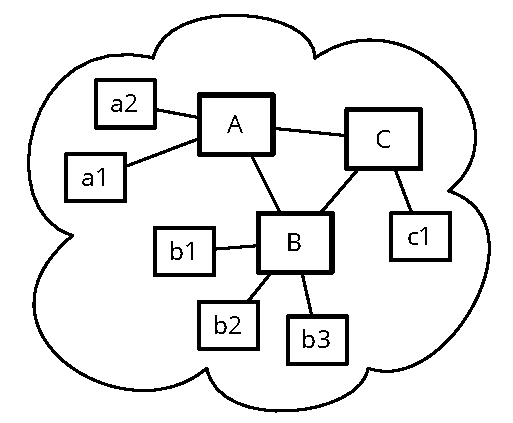
\includegraphics[width=0.5\textwidth]{/Users/ducasse/Workspace/FirstCircle/MyBooks/Bk-Writing/PharoBooks/LearningOOPWithPharoTrans/_result/pdf/Chapters/SimpleLAN/figures/lan-routes.pdf}\caption{A possible extension: a more realistic network with a cycle between three router nodes. \label{routing}}\end{center}
\end{figure}


Here is a possible setup for a new family of tests. 

\begin{displaycode}{smalltalk}
KARoutingNetworkTest >> buildNetwork
    | routers |
    net := KANetwork new.

    routers := #(A B C) collect:
        [ :each | KANetworkHub withAddress: each ].
    net connect: routers first to: routers second.
    net connect: routers second to: routers third.
    net connect: routers third to: routers first.

    #(a1 a2) do: [ :addr |
        net connect: routers first
            to: (KANetworkNode withAddress: addr) ].
    #(b1 b2 b3) do: [ :addr |
        net connect: routers second
            to: (KANetworkNode withAddress: addr) ].
    net connect: routers third
        to: (KANetworkNode withAddress: #c1)
\end{displaycode}


% lulu requires an empty page at the end. That's why I'm using
% \backmatter here.
\backmatter

% Index would go here
\bibliographystyle{abbrv}
\bibliography{others.bib}
\end{document}
